\documentclass[10pt,a4paper]{report}
\usepackage[utf8]{inputenc}
\usepackage[russian]{babel}
\usepackage{amsmath}
\usepackage{amsfonts}
\usepackage{amssymb}
\usepackage{graphicx}
\renewcommand{\thesection}{\arabic{section}}
\setcounter{totalnumber}{10}
\setcounter{topnumber}{10}
\setcounter{bottomnumber}{10}
\renewcommand{\topfraction}{1}
\renewcommand{\textfraction}{0}
\author{Евсеев Дмитрий}
\title{Лабораторная работа №6.\\
	Утилита nmap}

\begin{document}
\maketitle
\tableofcontents
\pagebreak

\section{Цель работы}

Научиться работать с Nmap

\section{Описание}

\textbf{nmap} — свободная утилита, предназначенная для разнообразного настраиваемого сканирования IP-сетей с любым количеством объектов, определения состояния объектов сканируемой сети (портов и соответствующих им служб). Изначально программа была реализована для систем UNIX, но сейчас доступны версии для множества операционных систем.

Nmap использует множество различных методов сканирования, таких как UDP, TCP (connect), TCP SYN (полуоткрытое), FTP-proxy (прорыв через ftp), Reverse-ident, ICMP (ping), FIN, ACK, Xmas tree, SYN- и NULL-сканирование. Nmap также поддерживает большой набор дополнительных возможностей, а именно: определение операционной системы удалённого хоста с использованием отпечатков стека TCP/IP, «невидимое» сканирование, динамическое вычисление времени задержки и повтор передачи пакетов, параллельное сканирование, определение неактивных хостов методом параллельного ping-опроса, сканирование с использованием ложных хостов, определение наличия пакетных фильтров, прямое (без использования portmapper) RPC-сканирование, сканирование с использованием IP-фрагментации, а также произвольное указание IP-адресов и номеров портов сканируемых сетей.

Для проведения работы будем использовать две виртуальные машины:

\begin{itemize}
	\item Kali linux для поиска и эксплуатации уязвимостей. IP: 172.16.105.134
	\item Metasploitable2 для тестирования. IP 172.16.105.135
\end{itemize}

\section{Ход работы}

\subsection{Поиск активных хостов}

Сканируем локальную сеть и ищем активные хосты с помощью команды nmap с ключом -sn и диапазоном ip адресов (рисунок \ref{Img:1}).
\begin{verbatim}
$ nmap -sn 127.16.105.0/24
\end{verbatim}

\begin{figure}[h!]	
	\center{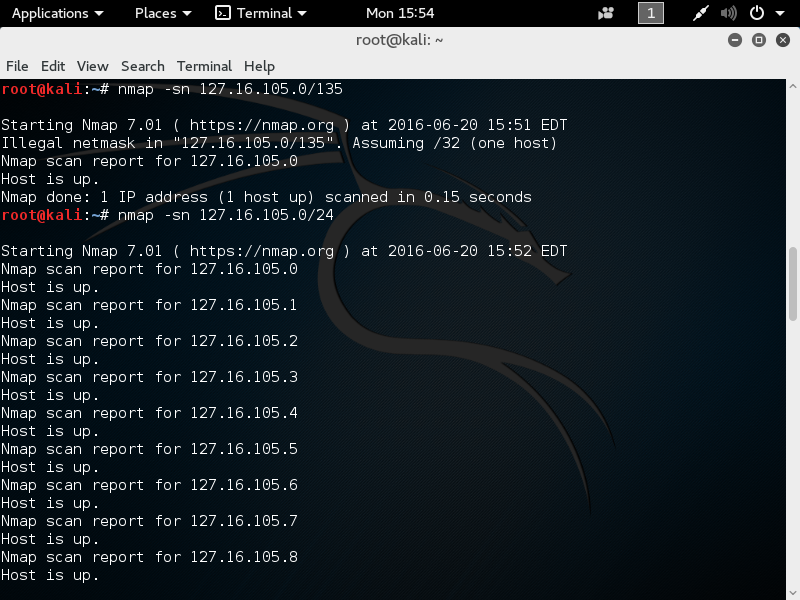
\includegraphics[width=0.8\linewidth]{Img/1}}
	\caption{Поиск активных хостов.}
	\label{Img:1}
\end{figure}
\pagebreak

\subsection{Определение открытых портов}

Для определения открытых портов необходимо воспользоваться следующей командой (рисунок \ref{Img:2})
\begin{verbatim}
$ nmap --open [hostIP]
\end{verbatim}

\begin{figure}[h!]	
	\center{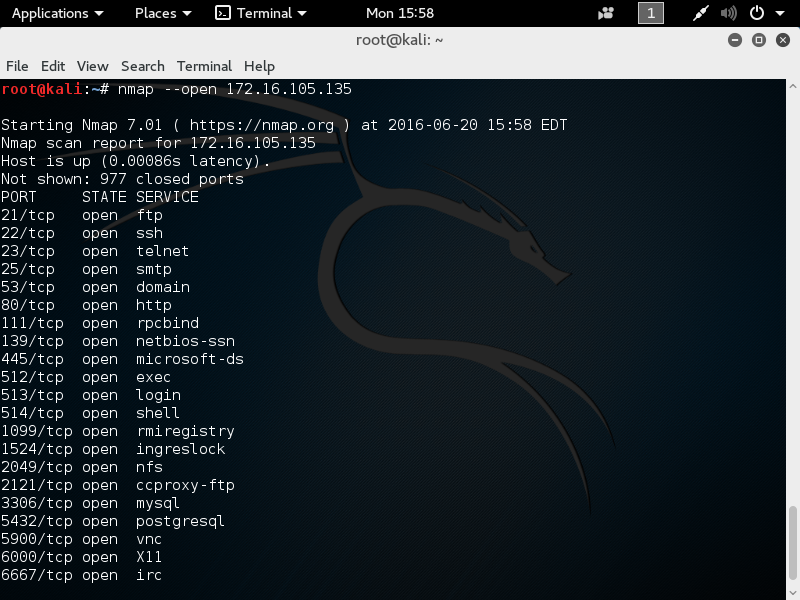
\includegraphics[width=0.8\linewidth]{Img/2}}
	\caption{Определение открытых портов.}
	\label{Img:2}
\end{figure}

\subsection{Определение версий сервисов}

Для определения открытых портов необходимо воспользоваться следующей командой (рисунок \ref{Img:2})
\begin{verbatim}
$ nmap --open [hostIP]
\end{verbatim}

\begin{figure}[h!]	
	\center{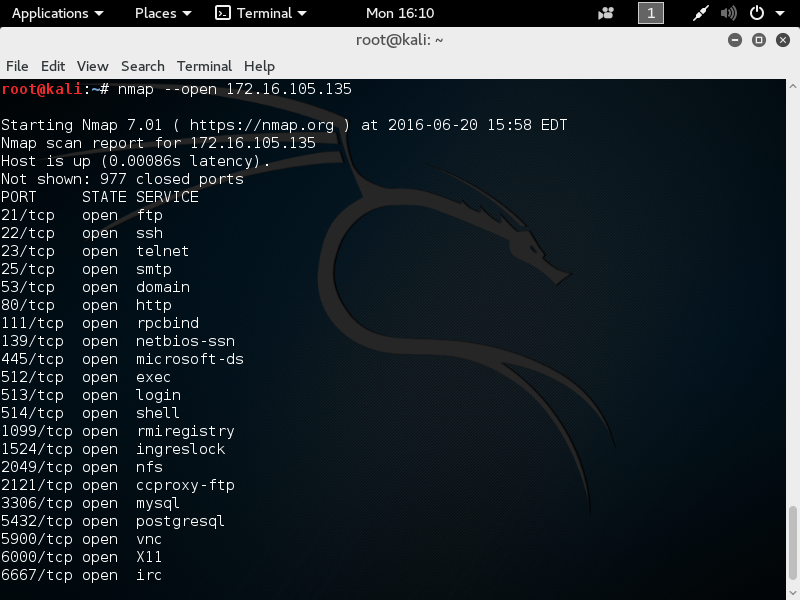
\includegraphics[width=0.8\linewidth]{Img/3}}
	\caption{Определение версий сервисов.}
	\label{Img:3}
\end{figure}

\subsection{Исследование служебных файлов nmap-services, nmap-os-db, nmap-service-probes}

Служебные файлы для утилиты nmap по умолчанию располагаются в директории "/usr/share/nmap".

\paragraph{nmap-services\\}

Служебный файл nmap-services содержит в себе описание назначения стандартных портов. Сам файл имеет структуру таблицы со следующими столбцами: имя сервиса, номер порта, название протокола, вероятность того, что порт открыт, комментарии.

Для известных зарезервированных номеров портов, файл содержит подробное описание. Пример на рисунке \ref{Img:4}.

\begin{figure}[h!]	
	\center{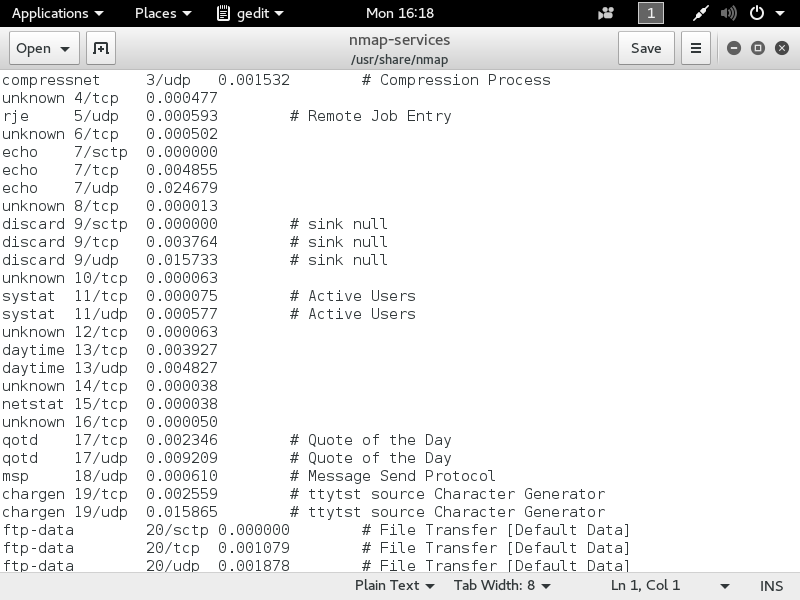
\includegraphics[width=0.8\linewidth]{Img/4}}
	\caption{Содержимое файла nmap-services.}
	\label{Img:4}
\end{figure}
\pagebreak

\paragraph{nmap-os-db\\}

Данный файл необходим для определения ОС хоста. В ней содержится примеры ответов различных ОС на специальные запросы Nmap. Он разделен на блоки, так называемые отпечатки, содержащие название ОС, классификацию и данные ответа.  Пример для ОС Linux на рисунке \ref{Img:5}.

\begin{figure}[h!]	
	\center{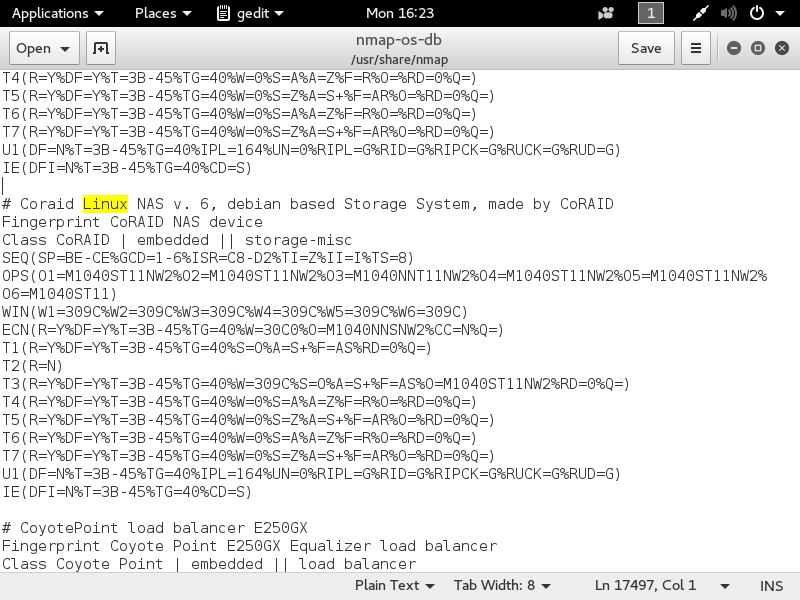
\includegraphics[width=0.8\linewidth]{Img/5}}
	\caption{Содержимое файла nmap-os-db.}
	\label{Img:5}
\end{figure}

\paragraph{nmap-service-probes\\}

Этот файл содержит "пробы", используемые для определения программ по прослушиваемому порту (ключи -sV и -A). Данный о сервисах задаются при помощи нескольких директив:
\begin{itemize}
	\item Exclude <port specification>
	\item Probe <protocol> <probename> <probestring>
	\item match <service> <pattern> [<versioninfo>]
\end{itemize}

Пример для mysql:

\begin{figure}[h!]	
	\center{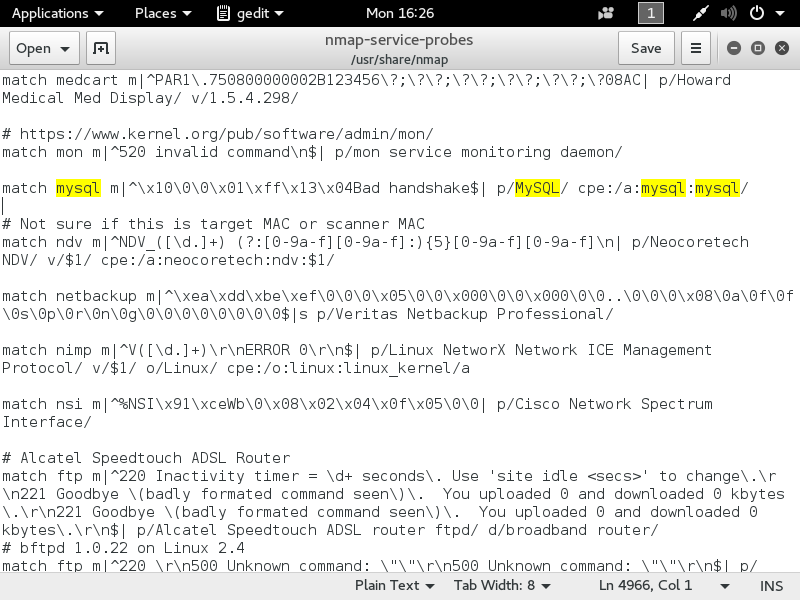
\includegraphics[width=0.8\linewidth]{Img/6}}
	\caption{Содержимое файла nmap-service-probes.}
	\label{Img:6}
\end{figure}

\subsection{Создание собственной сигнатуры}

Попробуем добавить собственную сигнатуру в файл nmap-service-probes. Для этого напишем простейший сервер, который слушает порт 22000 и на входящее сообщение отправляет приветственное сообщение со своей версией (Исходный код находится в файле tcpserver.c). 

Для определения данного сервера, добавим в файл nmap-service-probes следующие строки:

\begin{verbatim}
Probe TCP MyServer q|\x02Hi|
rarity 1
ports 22000
match testServer m/^Hello, client \((\w*) ([\d.]*)\)/ p/$1/ v/$2/
\end{verbatim}

В данных строках мы описываем, какое сообщение будем отправлять для идентификации, на какой порт, а так же какой ответ мы будем ожидать.

Запустим сканирование интересующего нас порта. Результат показан на рисунке \ref{Img:7}

\begin{figure}[h!]	
	\center{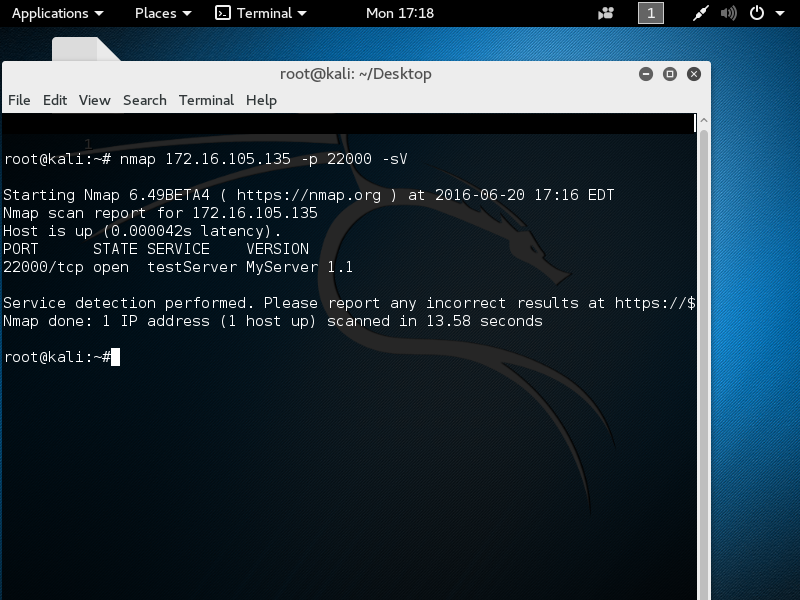
\includegraphics[width=0.8\linewidth]{Img/7}}
	\caption{Обнаружение тестовой утилиты.}
	\label{Img:7}
\end{figure}

\subsection{Сохранение вывода в xml}

Для сохранения вывода утилиты в файл xml необходимо воспользоваться \textbf{-oX <file>}. Например,

\begin{verbatim}
nmap -sV 127.16.105.135 -oX /home/nmap_sv_1.xml
\end{verbatim}

\subsection{Исследование работы Nmap с помощью Wireshark}
\label{wireshark}

Для исследования сетевой активности nmap воспользуемся утилитой Wireshark. Для примера отследим пакеты относящиеся к определения TCP сервиса, написанного нами ранее.

На Рисунках \ref{Img:8}, \ref{Img:9} отображены TCP пакеты для определения версии сервиса. В исходящем пакете в передаваемых данных можно наблюдать текст "it\_it\_test\_tcp\_server", а в ответном пакете - "yes\_it\_is".

\begin{figure}[h]
	\begin{center}
		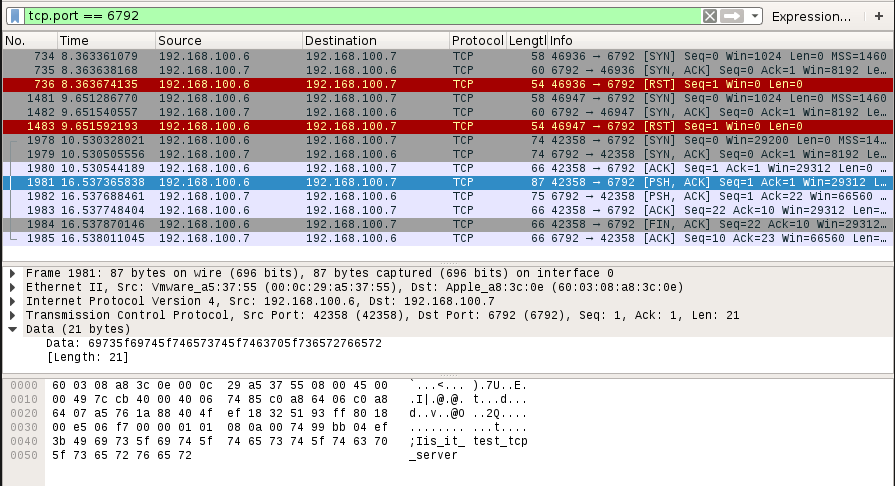
\includegraphics[width=0.65\textwidth]{Img/8}
		\caption{Исходящий TCP пакет.}
		\label{Img:8}
	\end{center}
\end{figure}

\begin{figure}[h]
	\begin{center}
		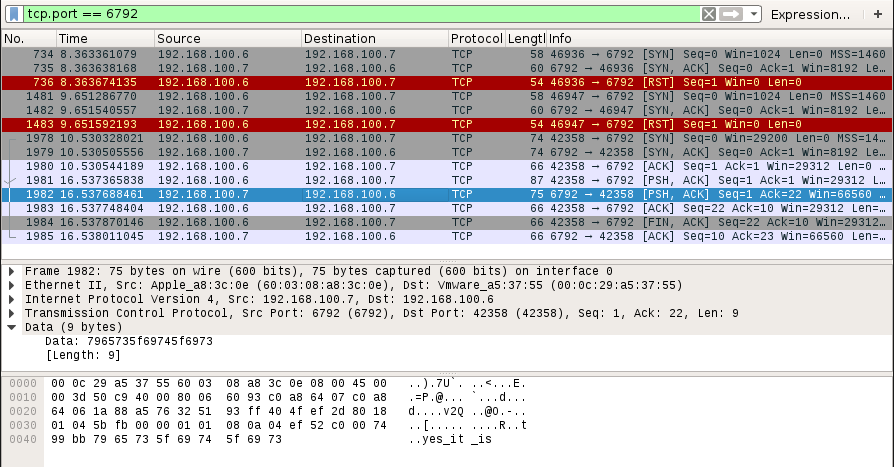
\includegraphics[width=0.65\textwidth]{Img/9}
		\caption{Входящий TCP пакет.}
		\label{Img:9}
	\end{center}
\end{figure}

\subsection{Metasploit Framework}
\label{msf}

- инструмент для создания, тестирования и использования эксплойтов. Позволяет конструировать эксплойты с необходимой в конкретном случае «боевой нагрузкой» (payloads), которая выполняется в случае удачной атаки, например, установка shell или VNC сервера. Также фреймворк позволяет шифровать шеллкод, что может скрыть факт атаки от IDS или IPS. Для проведения атаки необходима информация об установленных на удаленном сервере сервисах и их версии, то есть нужно дополнительное исследование с помощью таких инструментов, как nmap или nessus.

Проверим на уязвимости виртуальную машину Metasploitable2, используя db\_nmap (аналог nmap, сохраняющий результаты в БД) командой

\begin{verbatim}
db_nmap -A 192.168.100.9
\end{verbatim}

Результат сканирования отображен на Рисунках \ref{Img:10}, \ref{Img:11}, \ref{Img:12}

\begin{figure}[h]
	\begin{center}
		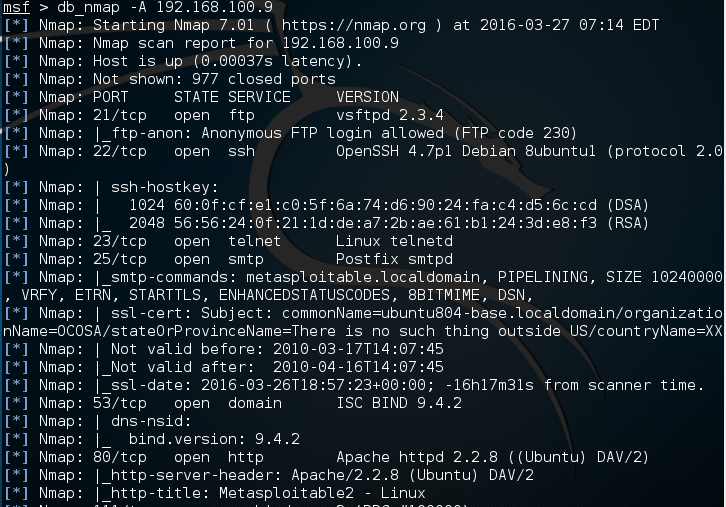
\includegraphics[width=0.8\textwidth]{Img/10}
		\caption{db\_nmap}
		\label{Img:10}
	\end{center}
\end{figure}

\begin{figure}[h]
	\begin{center}
		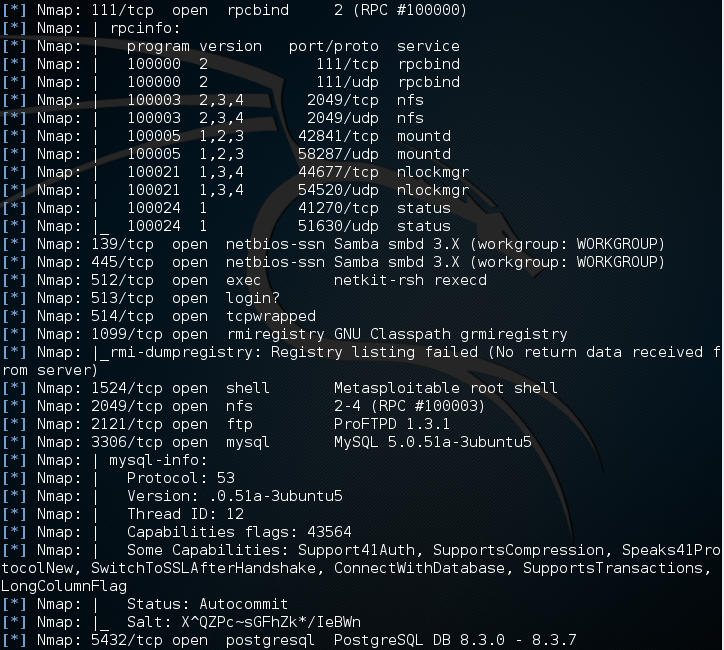
\includegraphics[width=0.8\textwidth]{Img/11}
		\caption{db\_nmap}
		\label{Img:11}
	\end{center}
\end{figure}

\begin{figure}[h]
	\begin{center}
		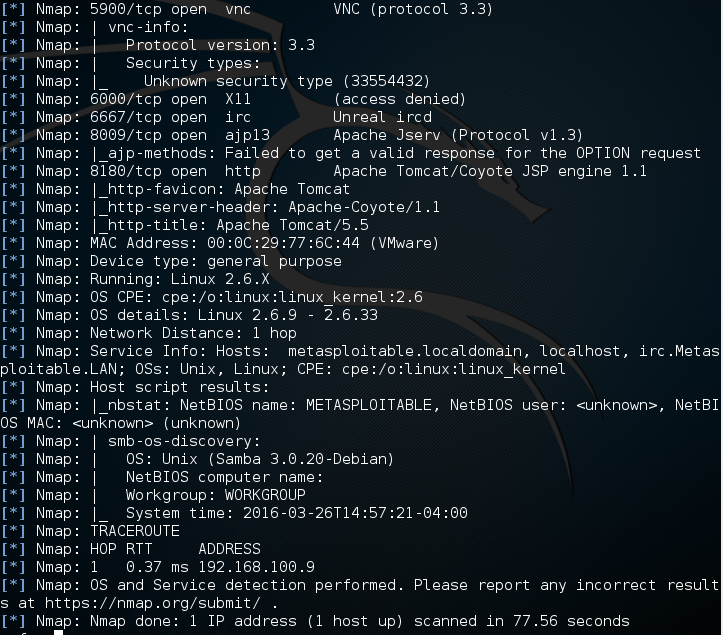
\includegraphics[width=0.8\textwidth]{Img/12}
		\caption{db\_nmap}
		\label{Img:12}
	\end{center}
\end{figure}

\subsection{Примеры записей из nmap-service-probes}
\label{probes_example}

\begin{verbatim}
##############################NEXT PROBE##############################
# Detects TN3270 Servers which send IAC DO TTYPE on initial connection
# instead of IAC DO TN3270E
Probe TCP tn3270 q|\xff\xfb\x18\xff\xfa\x18\x00IBM-3279-4-E\xff\xf0|
rarity 8
ports 23,2323,2023,623
sslports 992
\end{verbatim}

Согласно данной записи nmap для обнаружения сервиса использует протокол tcp для отправки пакета, содержащего \begin{verbatim}\xff\xfb\x18\xff\xfa\x18\x00IBM-3279-4-E\xff\xf0\end{verbatim}
Целевые порты 23, 2323, 2023, 623, ssl - 992. rarity - индикатор того, насколько часто возвращаемые пакеты содержат полезную информацию.

\begin{verbatim}
##############################NEXT PROBE##############################
Probe UDP AndroMouse q|AMSNIFF|
rarity 9
ports 8888

match AndroMouse m|^GOTBACK$|s p/AndroMouse Android remote mouse server/
\end{verbatim}

Протокол - UDP, редкость полезных ответов - 9, порт - 8888.
Данные для отправки \begin{verbatim}AMSNIFF\end{verbatim}
Шаблон ответа \begin{verbatim}m|^GOTBACK$|s\end{verbatim}
Дополнительная информация - "AndroMouse Android remote mouse server"

\begin{verbatim}
##############################NEXT PROBE##############################
Probe UDP AirHID q|from:airhid|
rarity 9
ports 13246
match AirHID m|^andReceiver-\d+\.\d+\.\d+$|s p/AirHID Andrioid remote mouse server/
\end{verbatim}

Протокол - UDP, редкость полезных ответов - 9, порт - 13246.
Данные для отправки \begin{verbatim}from:airhid\end{verbatim}
Шаблон ответа \begin{verbatim}m|^andReceiver-\d+\.\d+\.\d+$|s\end{verbatim}
Дополнительная информация - "AirHID Andrioid remote mouse server"

\begin{verbatim}
##############################NEXT PROBE##############################
# Queries z/OS Network Job Entry
# Sends an NJE Probe with the following information (text is converted to EBCDIC):
# TYPE        = OPEN
# OHOST       = FAKE
# RHOST       = FAKE
# RIP and OIP = 0.0.0.0
# R           = 0
# Based on http://www-01.ibm.com/support/knowledgecenter/SSLTBW_2.1.0/com.ibm.zos.v2r1.hasa600/init.htm
Probe TCP NJE q|\xd6\xd7\xc5\xd5@@@@\xc6\xc1\xd2\xc5@@@@\0\0\0\0\xc6\xc1\xd2\xc5@@@@\0\0\0\0\0|
rarity 9
ports 175
sslports 2252
# If the port supports NJE it will respond with either a 'NAK' or 'ACK' in EBCDIC
match nje m|^\xd5\xc1\xd2| p/IBM Network Job Entry (JES)/
match nje m|^\xc1\xc3\xd2| p/IBM Network Job Entry (JES)/
\end{verbatim}

Протокол - TCP, редкость полезных ответов - 9, порт - 175, ssl порт - 2252.
Данные для отправки \begin{verbatim}\xd6\xd7\xc5\xd5@@@@\xc6\xc1\xd2\xc5@@@@\0\0\0\0\xc6\xc1\xd2\xc5@@@@\0\0\0\0\0\end{verbatim}
Шаблоны ответа 
\begin{verbatim}
\xd5\xc1\xd2
\xc1\xc3\xd2
\end{verbatim}
Дополнительная информация для обоих шаблонов - "IBM Network Job Entry (JES)"

\begin{verbatim}
##############################NEXT PROBE##############################
# Sends a ServerInfo PBC request to the Basho Riak distributed database
Probe TCP riak-pbc q|\0\0\0\x01\x07|
rarity 8
ports 8087
match riak-pbc m|^....\x08..(riak@[\w._-]+)..([\w._-]+)$|s p/Basho Riak/ v/$2/ h/$1/
\end{verbatim}

Протокол - TCP, редкость полезных ответов - 8, порт - 8087.
Данные для отправки \begin{verbatim}\0\0\0\x01\x07\end{verbatim}
Шаблоны ответа 
\begin{verbatim}
^....\x08..(riak@[\w._-]+)..([\w._-]+)$
\end{verbatim}
Дополнительная информация - "Basho Riak", версия и имя хоста получаются из регулярного выражения.

\subsection{Описание скрипта finger}
\label{finger_script}

В начале содержится описание скрипта

\begin{verbatim}
description = [[
Attempts to get a list of usernames via the finger service.
]]

author = "Eddie Bell"

license = "Same as Nmap--See https://nmap.org/book/man-legal.html"
\end{verbatim}

Категории, к которым принадлежит скрипт

\begin{verbatim}
categories = {"default", "discovery", "safe"}
\end{verbatim}

Пример вывода

\begin{verbatim}
---
-- @output
-- PORT   STATE SERVICE
-- 79/tcp open  finger
-- | finger:
-- | Welcome to Linux version 2.6.31.12-0.2-default at linux-pb94.site !
-- |  01:14am  up  18:54,  4 users,  load average: 0.14, 0.08, 0.01
-- |
-- | Login      Name                  Tty      Idle  Login Time   Where
-- | Gutek      Ange Gutek           *:0          -     Wed 06:19 console
-- | Gutek      Ange Gutek            pts/1   18:54     Wed 06:20
-- | Gutek      Ange Gutek           *pts/0       -     Thu 00:41
-- |_Gutek      Ange Gutek           *pts/4       3     Thu 01:06
\end{verbatim}

Подлючение библиотек

\begin{verbatim}
require "comm"
require "shortport"
\end{verbatim}

Проверка называется ли сервис "finger" или порт равен 79. 
\begin{verbatim}
portrule = shortport.port_or_service(79, "finger")
\end{verbatim}

nmap.new\_try создает обработчик исключений, comm.exchange - обрабатывает сетевые транзакции. В данном случае просиходит ожидание пока не получено хотя бы 100 строк, не менее 5 секунд или пока хост не закроет подлючение.

\begin{verbatim}
action = function(host, port)
local try = nmap.new_try()

return try(comm.exchange(host, port, "\r\n",
{lines=100, proto=port.protocol, timeout=5000}))
end
\end{verbatim}

\newpage

\section{Вывод}

В результате выполнения работы изучена утилита nmap. С помощью нее были просканированы хосты на уязвимости. Работа nmap была изучена с помощью утилиты Wireshark. Так же произведено знакомство с Metasploit framework.


\end{document}